\label{chap:BasicPrin}
\section{Deep Neural Networks}

To clearly explain what an Autoencoder is, we must first lay the foundations of one of its core concepts: \textbf{Deep Neural Networks}. DNN constitute the basis of Deep Learning and they have proven themselves to be complex enough to tackle many of the data challenges of today. \par

\begin{figure}[H]
	\begin{subfigure}{0.65\linewidth}  
		\centering
		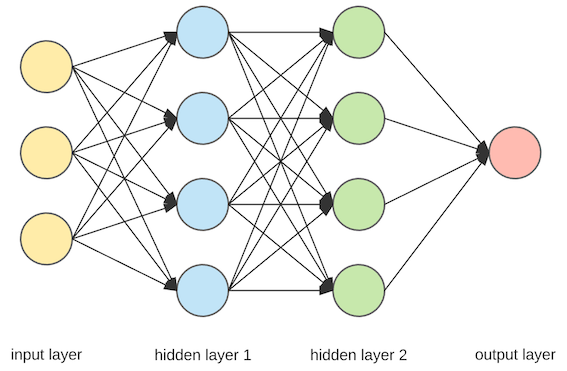
\includegraphics[width=\linewidth]{Figuras_tfg/Figure2_tfg}
		\caption{Basic depiction of a simple DNN composed by two hidden layers and a single 2-input/1-output system.}
		\label{fig:fig2a} 
	\end{subfigure}
	
	\begin{subfigure}{0.65\linewidth} 
		\centering
		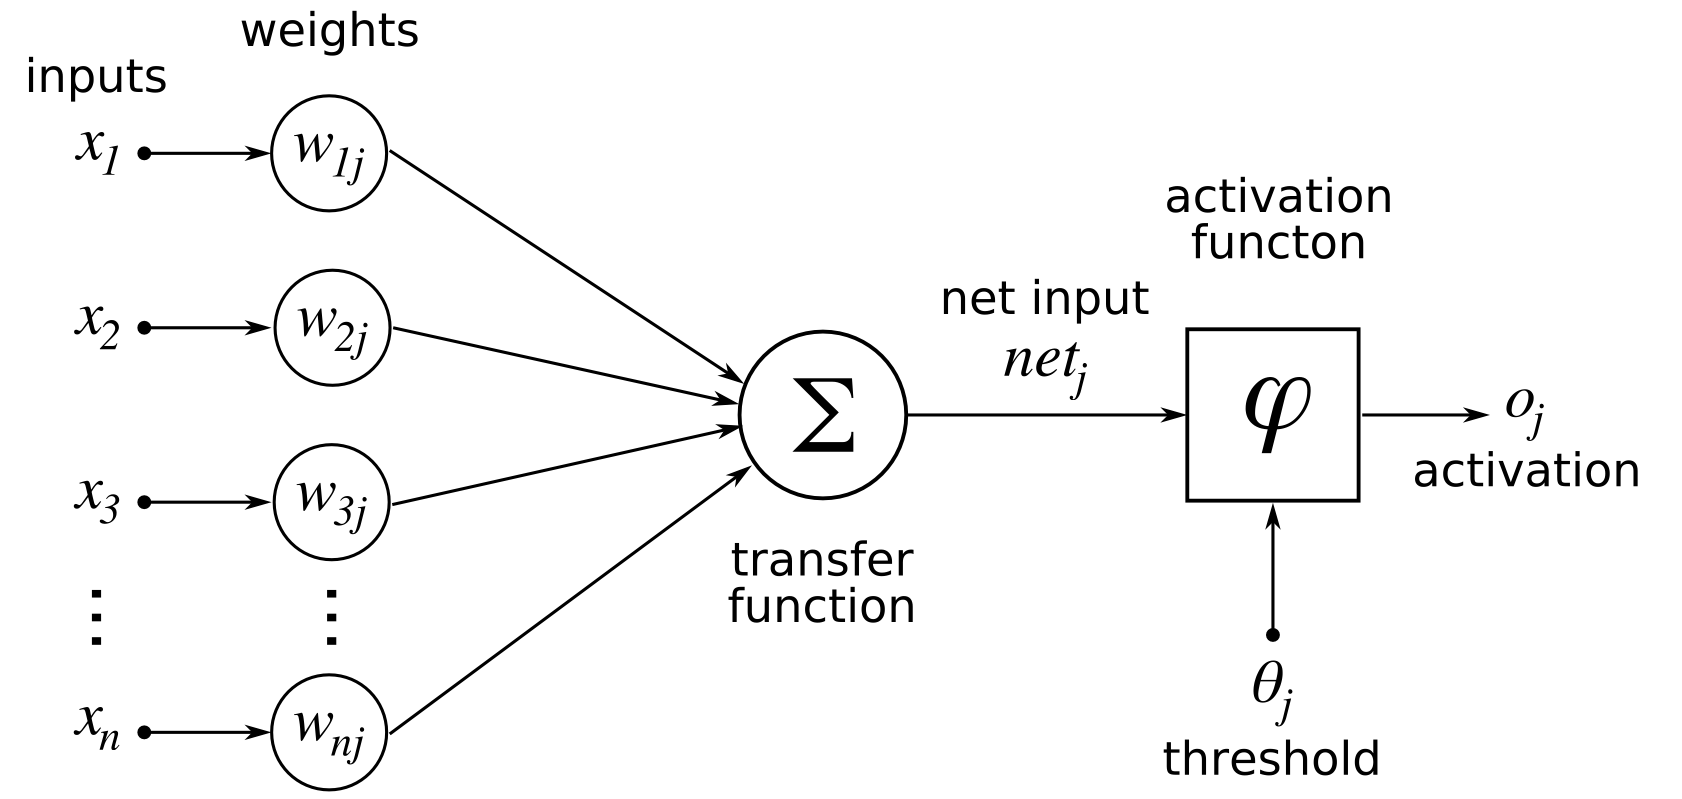
\includegraphics[width=\linewidth]{Figuras_tfg/ArtificialNeuronModel_english.png}
		\caption{Normal architecture of an artificial neuron.}
		\label{fig:fig2b} 
	\end{subfigure}
	\caption{Basic depiction of a simple DNN composed by two hidden layers and a single 2-input/1-output system.}
	\label{fig:fig2}
\end{figure}

By analysing Figure2a, it can be noted that DNNs are comprised of multiple layers of units (or neurons) with a relatively small computing power which is calculated using the weights from previous layers combined with an activation function as seen on and \ref{fig:fig2}. It also has an input (usually denoted as X) which is feed-forwarded to the hidden layers in the network and subsequently transformed into an output (commonly denoted as Y). 

\begin{equation}\label{eq:artificial neuron}
Output = f( bias_j + \sum_{i = 0}^{n} w_{i}*x_i ) 
\end{equation}


Neurons inside of the network can be modeled according to different types, although in this report we will be only taking into account two of them: the sigmoid $f(x) = \frac{1}{1 - e{-x}}$ (Figure a) and the relu $f(x) = max(0,x)$(Figure b) neurons. I chose to use this type of neurons because their activation functions are excellent for minimizing the reconstruction loss inside of the Autoencoder. \newline

\begin{figure}[H]
	\begin{minipage}{.5\textwidth}
		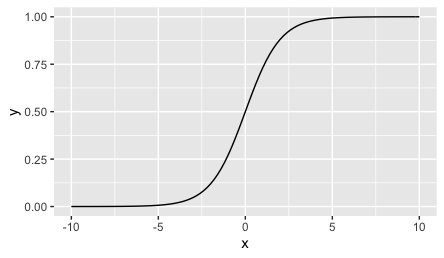
\includegraphics[scale=.5]{Sigmoid_function}
	\end{minipage}%
	\begin{minipage}{.5\textwidth}
		\begin{flushright}
			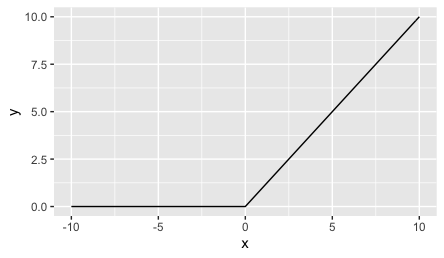
\includegraphics[scale=.5]{Relu_function}  
		\end{flushright} 
	\end{minipage}  
	\caption{The left graph represents a Sigmoid function, while on the right there is a Relu function}
	\label{fig:fig3}
\end{figure}

As it can be seen on Figure\ref{fig:fig3} , the Relu function has a relatively simple representation, which makes it less computationally expensive when compared with the Sigmoid. The Sigmoid function takes values between 0 and 1, which makes it specially useful when we want to place a classifier as the next task after the transformation.\par 

Once a certain DNN structure has been activated, the neurons inside of the network will start to propagate the information through it in a non-linear manner in order to try to achieve a given established task, which in our particular case consists in transforming the representation of our input into a smaller but informationally more compressed form. Other experts can use the same principles to achieve other goals including decision-making, visualization,....etc.\par

\section{Information Bottleneck Principle}

The architecture of the Autoencoder is based upon the IB, a method proposed in \cite{Inf_Bottleneck_first} whose principle relies on extracting the relevant information that an input random variable X contains about another output random variable Y. If we assume that there is some type of statistical dependency between X and Y, the relevant information can be defined as $I(X;Y)$.\par

\begin{figure}[H]
	\centering
	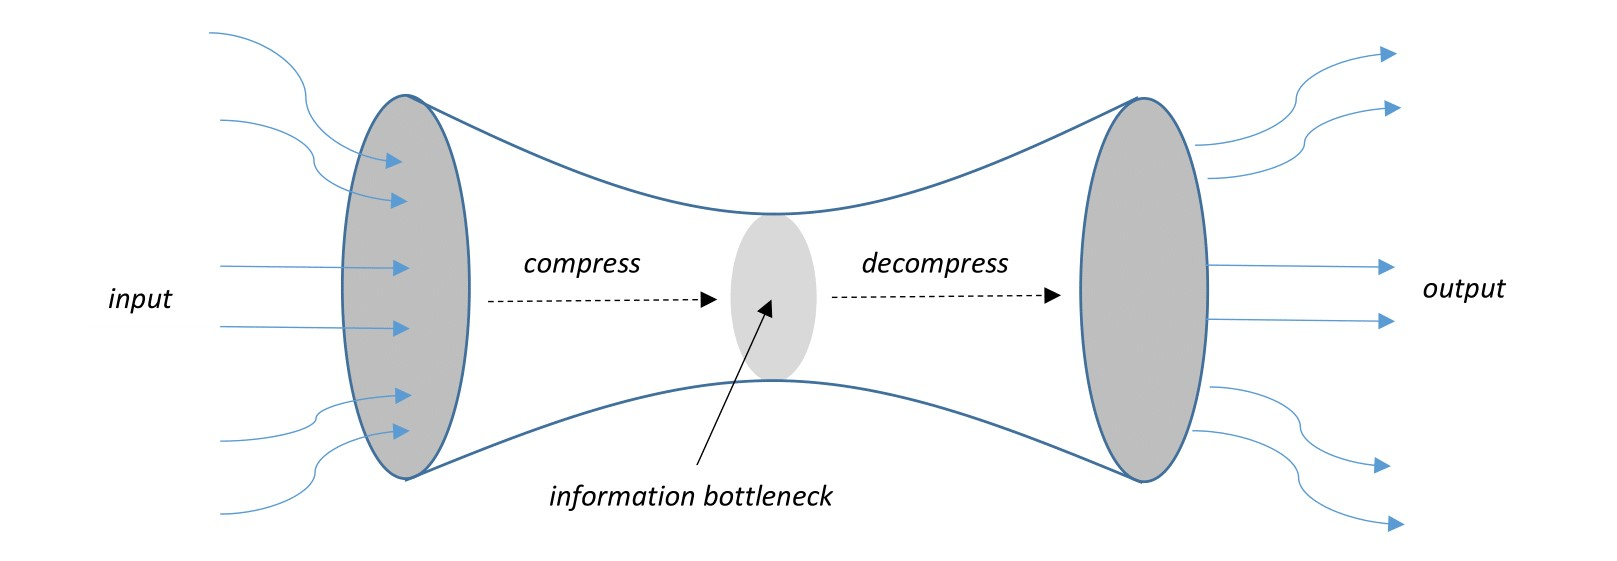
\includegraphics[width=\linewidth]{Informational_Bottleneck.jpg}
	\caption{Concept drawing of the Information Bottleneck.}
	\label{fig:figure_info_bottle}
\end{figure} 

If we want to obtain the optimal representation of X, we would want to capture the relevant information of X that contributes to an accurate prediction of Y. This term is known as the \textbf{minimal sufficient statistics}, or simply just the mapping of X that retains $I(X;Y)$. The compressed version of $X$ is denoted as $T$, and we can analyze the accuracy of our compression by comparing the prediction of $Y$ that both $T$ and $X$ do. Essentially,our goal is to fulfill the following equation: \newline 

\begin{equation}\label{eq:Bottleneck_equation}
\min\limits_{p(t|x)}  I(X;T) - \beta \times I(T;Y)
\end{equation} \newline

During the compressing process, and as depicted in Figure \ref{fig:figure_info_bottle}, DNNs only have access to the information that has been transferred to them via the previous layers of the system. This has a big effect on our network: the information not processed on the last immediate layer is essentially lost. This is the main reason why every layer should attempt to maximize $I(Y;hi)$ while trying to minimize $I(hi-1;hi)$, being $hi$ a random layer situated inside of the coding or compressing layer and $hi-1$ its immediate predecessor. Here, it is important to consider then that we want to reduce the length of the layer to the minimum possible without affecting the predictive features of our model. \par

Each layer of our model should require shorter descriptions than the previous ones, being the first one with the longest description and the least compression. It must also be noted that every model will require a different set of layers and an architecture to fit its computational needs to the optimal level. \par

\section{The Autoencoder}

\subsection{The Autoencoder Architecture}

Applying the concepts introduced on both of the previous sections, the Autoencoder comes as a mixture of them. Figure \ref{fig:figure_autoencoder} below presents it as a three part structure: A encoder, the middle layer and finally the decoder. \par

\begin{figure}[H]
 \centering
  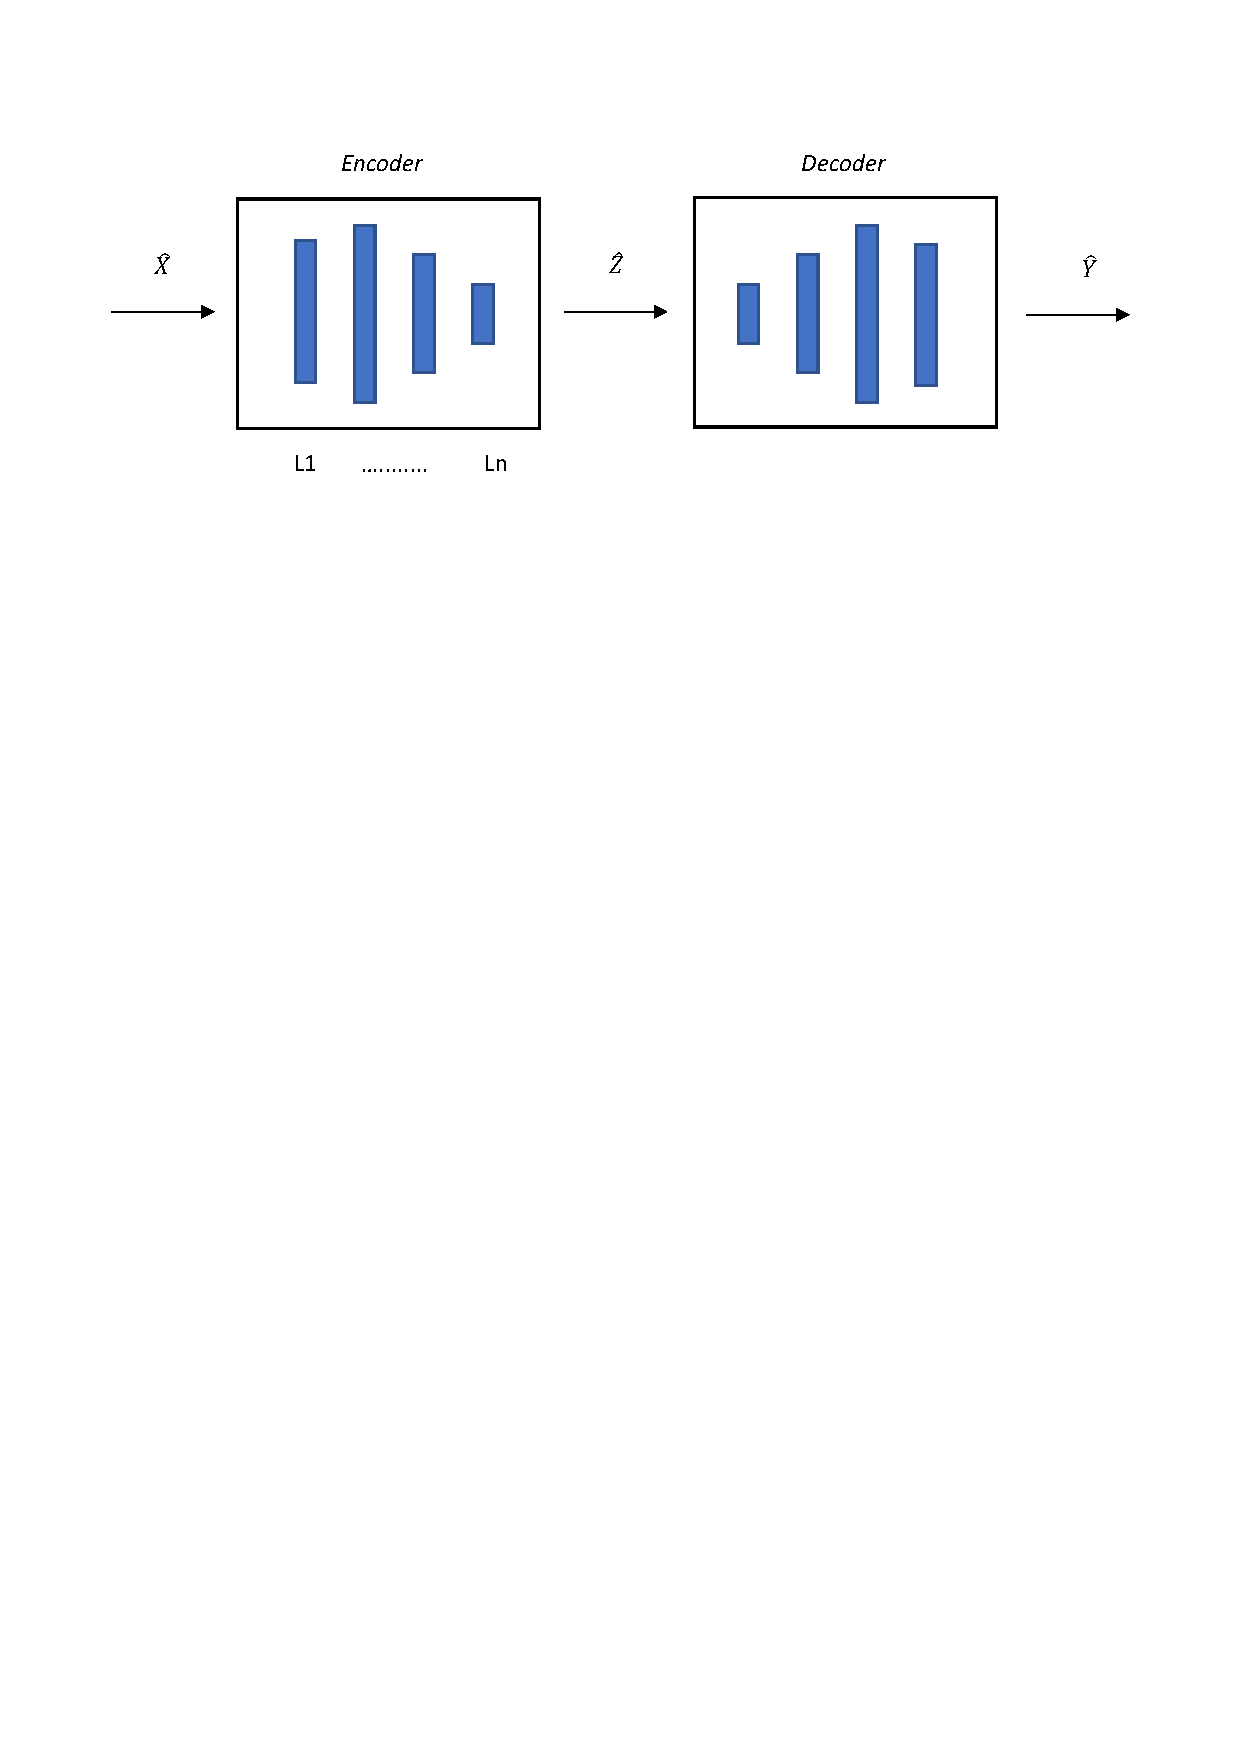
\includegraphics[width=16cm]{Figuras_tfg/Figura_autoencoder}
  \caption{Taking into account the Figure \ref{fig:fig1a}, this diagram depicts the inside of the transformation box. Both the Encoder and the Decoder have symmetric shapes, as well as an expansion layer (the second one in the encoder, the previous one in the decoder) whose goal is to separate the qualities of our data as sort of a preparation for the compression.}
 \label{fig:figure_autoencoder}
\end{figure} 

The theory of the Autoencoder has been around since the 1980s \ref{Autoencoders_first_mention}. As seen in Figure \ref{fig:figure_autoencoder}, the goal of the Autoencoder is not only to copy the input data and then transmit it through the network, but to retain the most important features of the data fed to it and to try to optimize the process of learning them. For the purpose of my research, I will only be considering the back-propagated Autoencoders, although it must be noted that other variances of them exist, such as the recirculated Autoencoders. \par

In our case, we will be also using an under-complete Autoencoder. Most of the types an Autoencoder is implemented it is usually more interesting to focus on its data compression capabilities rather than trying to copy the input onto the output. That is why we want to force the Autoencoder to provide us with a smaller dimension on the input data X in the output on the encoder, which for the purpose of this report we will denominate as $Z$. The learning process tries to minimize the given equation: \par

\begin{equation}\label{eq:artificial neuron}
L(x,g(f(x)))
\end{equation}

Being L a loss function that penalizes $g(f(x))$ for being dissimilar from $x$.

One thing to take into account when designing an Autoencoder is that giving too much capacity to its layers can be counterproductive to the learning task. This means that when given too much capacity to work with they will tend to learn to avoid extracting information and rather to just copy the information, which is an undesirable outcome. On the other hand, trying to set an encoder to code the input signal into a single dimension could result in the loss of valuable information. Even with a very powerful decoder a very optimized Autoencoder will struggle to perform this task, specially when introducing very big sets data as the input. \par

Taking into account this description, the general rule to design them is just by using trial and error. As we will see on \ref{chap:Result}, where I will be discussing the implementation of the Autoencoder, you can try different setups to reach the optimum middle layer size which accomplishes that there is no trade-off between augmenting its size and keeping its actual capabilities. The Tensorflow python tool provides us with the accuracy and loss variables that the Autoencoder is generating on each training epoch to check if your architecture is fulfilling your requirements. For the purpose of this report, we will not only taking into account those parameters, but we will also be using a tool to ensure that it transferring the higher quantity of information possible: \textbf{The Entropy Triangle}.

\subsection{The Entropy Triangle}
\subsubsection{Introduction}

In the previous section I have talked about how accuracy can be used to asses the validity of our model. In reality, the accuracy value can be somewhat misleading depending of the task that we are implementing it to check if we are carrying out our data analysis correctly. This statement is specially true when talking about Classification.\par

The usage of data classification has greatly improved in the past years. Nowadays, there are multiple papers discussing how it can be used in a wide range of topics, from the medical field \cite{Medical_Classification} to face recognition \cite{Balaban_2015} . That is why it is specially important to correctly address the scope of your task and characteristics of your variables to be able the get the maximum performance out of your predictions.\par

\begin{figure}[H]
 \centering
  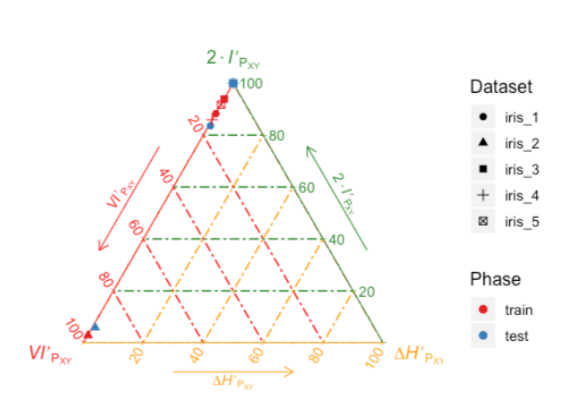
\includegraphics[width=15cm]{Figuras_tfg/Example_ET}
  \caption{Example of use of a typical Entropy Triangle. In this case, a Knn classification method is being tested in the triangle.}
 \label{fig:figure_example_et}
\end{figure} 

The real question comes when you have your results and you try to wrap your mind around them. In \cite{val:pel:14a} a very important reality is shown: the accuracy performance criterion is a very intuitive but ineffective tool. Another highly important concept is introduced here: the accuracy paradox.\par  

The accuracy paradox shows some of the defects that classifiers have been presenting for a long time now . For example, in some cases predictive classifiers which have given a lower accuracy power have also proven to display a higher predictive accuracy that other with a higher accuracy. The reason being most of the times is that we have trained our classifier with a single class that contains the majority of the data. In those cases, our classifier will just assign all of the input values to belong to the majority class since that is where the greater probability lies upon. This one is a very easily identifiable case of an imbalanced training data set. Moreover, since most of the times our data is gathered in controlled conditions, we risk the problem of this issue showing up more than we would wish to.\par

Once it is realized that the methods previously employed can lead to disingenuous results, a new realization arises: there is a need for a better measure of the classifier. As seen in, the Entropy Triangle and its features show some numeric example that fit the requirements and scope of our task, so I will be using it. Bur firstly, I will explain the basics of its functionalities.\par

\subsubsection{Architecture}

The Entropy Triangle was introduced in \cite{val:pel:10b} as a way of solving the problems presented in the previous sections. We consider the transmission of information through a channel as two random variables, named X for the input and Y for the output. Note that on Figure\ref{fig:fig1} we used a different naming standard, K and $\hat{K}$, but the new reference names are now implemented for the sake of easier computations. In Figure \ref{fig:figure_diagram_et} we can see a classical information-diagram which simply show the entropy relationship between X and Y or $P_xy$. From that Figure we can also asses some equations from it:\par

The Mutual Information, which quantifies the stochastic force between $P_X$ and $P_Y$ appears twice in the diagram both as:
\begin{equation}\label{eq:mutual_information_1}
MI_{P_{XY}} = H_{P_X * P_Y} - H_{P_{XY}}
\end{equation}
and,
\begin{equation}\label{eq:mutual_information_2}
MI_{P_{XY}} = H_{P_X} - H_{P_{X|Y}}
\end{equation}

The Virtual Information or variation of information are embodied by the sum of the two red areas and represents the residual entropy, which is not used in the binding of the variables:

\begin{equation}\label{eq:virtual_information}
VI_{P_{XY}} = H_{P_{Y|X}} + H_{P_{X|Y}}
\end{equation}

And both equations mentioned before together with $\Delta H_{P_{X} * P_{Y}}$, which represents the divergence between the joint distribution where $P_X$ and $P_Y$ are independent and the uniform distributions with the same cardinality of events as the previously mentioned $P_X$ and $P_Y$, form:

\begin{equation}\label{eq:uniform_entropy_x_y}
H_{U_{X} * U_{Y}} = \Delta H_{P_{X} * P_{Y}} + 2 * MI_{P_{XY}} + VI_{P_{XY}}
\end{equation}

In which case $H_{U_{X} * U_{Y}}$ is the outer rectangle with both the uniform distributions of the input and the output.

Once we have obtained equation\ref{eq:uniform_entropy_x_y} we will normalize it using the  $H_{U_{X} * U_{Y}}$ and thus forcing the variables involved in our calculations to be bounded by 0 and 1, as it can be seen on:

\begin{equation}\label{eq:normalised_uniformed}
1 = \Delta'H_{P_{X} * P_{Y}} + 2 * MI'_{P_{XY}} + VI'_{P_{XY}} 
\end{equation}
Which also will wield the following equation:
\begin{equation}\label{eq:complex_space_equation}
0 \leq \Delta'H_{P_{X} * P_{Y}}, MI'_{P_{XY}}, VI'_{P_{XY}}  \leq 1
\end{equation}
\newline
\begin{figure}[H]
 \centering
  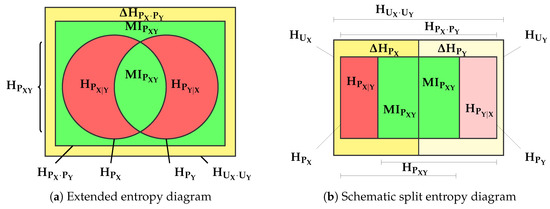
\includegraphics[width=14cm]{Figuras_tfg/ET_Diagram}
  \caption{Diagram representing an ET applied to a bi-variate distribution from \cite{val:pel:18c}.}
 \label{fig:figure_diagram_et}
\end{figure} 


By applying both equations \ref{eq:normalised_uniformed} and \ref{eq:complex_space_equation} we will get a point in the normalized space  $\Delta'H_{P_{X} * P_{Y}} x 2*MI'_{P_{XY}} x VI'_{P_{XY}}$. Each $P_{XY}$ can be characterized as $F(P_{XY}) = [\Delta'H_{P_{X} * P_{Y}},2*MI'_{P_{XY}},VI'_{P_{XY}}] $. The resulting diagram will be an equilateral triangle, where the coordinates are $F(P_{XY})$ and every bi-variate distribution is shown as a point in the diagram. Every zone of the triangle has certain characteristics related to it. \par

We can also divide equation \ref{eq:uniform_entropy_x_y} to obtain new representations of the split balance equations with respect to $X$ and $Y$,

\begin{equation}\label{eq:entropy_x_balance}
H_{U_{X}} = \Delta H_{P_{X}} + MI_{P_{XY}} + H_{P_{X|Y}}  -> 1 = \Delta H'_{P_{X}} + MI'_{P_{XY}} + H'_{P_{X|Y}}
\end{equation}
and,
\begin{equation}\label{eq:entropy_y_balance}
H_{U_{Y}} = \Delta H_{P_{Y}} + MI_{P_{XY}} + H_{P_{Y|X}}  -> 1 = \Delta H'_{P_{Y}} + MI'_{P_{XY}} + H'_{P_{Y|X}}
\end{equation}

Both equations are normalized by using both $H_{U_{X}}$ and $H_{U_{Y}}$ respectively. Now, we have new representations for $X$ and $Y$ in the 2-simplex triangle created before. The representation seems to split in two and have $F(P_X) = [\Delta'H_{P_{X}},MI'_{P_{XY}},H'_{P_{X|Y}}] $ and $F(P_Y) = [\Delta'H_{P_{Y}},MI'_{P_{XY}},H'_{P_{Y|X}}]$ coordinates.\newline

\begin{figure}[H]
 \centering
  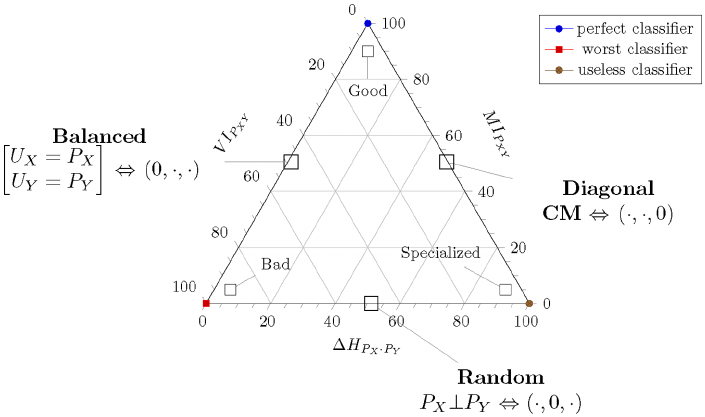
\includegraphics[width=15cm]{Figuras_tfg/ET_Labelled.png}
  \caption{From \cite{val:pel:18c} Schematic of an Entropy Triangle. The labels are placed close to the side of the triangle that is related to the feature mentioned in it.}
 \label{fig:figure_labelled_et}
\end{figure} 

Most of the equations included here can be found in \cite{val:pel:18c} which discusses most of the points mentioned here along with some examples of use and much more information on the tool and different implications of its use. \par

The triangle itself works as a great tool to characterize the performance of your model. The position of the coordinates assesses the quality of your classifier. It can be appreciated from Figure \ref{fig:figure_labelled_et} that classifiers which are at the apex or close to it obtain the highest accuracy possible on balanced datasets and transmit a lot of mutual information, which makes them the best classifiers possible. On the other hand, when the coordinates of the classifier are very close to the left apex, we will be working with balanced data but the classifier will be doing a very bad work with it, we are dealing with the worst classifier. Finally, those who are located at the right apex or close to it represent the accuracy paradox mentioned before, which a highly specialized classifier which tries to work with very unbalanced data.\par

One example of use of the Entropy Triangle would be to use the true labels $K$ and the predicted labels $\hat{K}$ to generate a confusion matrix. Using an algorithm, the entropy of the process is calculated according the values in the confusion matrix, which will then provide us with a coordinate inside of the ET. It will provide visual data to assess the feasibility of the task and its effectiveness.\par





